\documentclass[10pt, a4paper]{article}

\input{/home/mykhailo/.config/nvim/templates/preamble.tex}

\newcommand{\department}{ЗІ}
\newcommand{\reportnumber}{2}
\newcommand{\reporttitle}{Розробка консольних утиліт для задач кібербезпеки}
\newcommand{\profname}{Кебус В. М.}

\begin{document}

\input{/home/mykhailo/Documents/lpnu/report_title_page}
Мета:
\begin{enumerate}
	\item Закріпити та поглибити знання з об'єктно-орієнтованого програмування (ООП) в Python: створення класів, інкапсуляція, наслідування, композиція, спеціальні методи класів та декоратори \verb|@property|, \verb|@dataclass|.
	\item Опанувати роботу зі стандартною бібліотекою Python для обробки даних. Маніпуляція шляхами та файлами \verb|pathlib|, робота з форматами JSON та CSV, обробка дати і часу \verb|datetime|, використання спеціалізованих структур даних \verb|collections| та регулярних виразів \verb|re|.
	\item Навчитися будувати надійні та стійкі консольні програми (CLI-утиліти): обробка винятків, валідація вхідних даних, структуроване логування подій (\verb|logging|) та розбір аргументів командного рядка (\verb|argparse|).
\end{enumerate}
\section{План виконання роботи}
\begin{enumerate}
	\item Підготовка репозиторію та середовища: Продовжити використання репоизторію cybersecurity-python-labs, створити нову папку labs/lab02, оновити залежності
	\item Виконати завдання 1 (ООП): Реалізація системи моделювання користувачів, безпечних сесій та логування на основі класів.
	\item Виконати завдання 2 (Консольна утиліта кібербезпеки): Розробка повноцінної CLI-утиліти відповідно до варіанта за допомогою argparse, logging, pathlib, re та модулів обробки даних.
	\item Контроль якості коду через Ruff: перевірка та автоматичне форматування всього коду лабораторної роботи за допомогою ruff check та ruff format.
	\item Зберегти код у Git-репозиторії, Підготовка фінального звіту, збереження результатів та відповіді на контрольні запитання.
\end{enumerate}
\section{Завдання}
\subsection{Завдання 1: Модель користувача й облікового запису}
\textbf{Кроки виконання}
\begin{enumerate}
	\item \textbf{Віртуальне середовище.} Активуйте середовище з ЛР№1 та встановіть залежності проєкту командорю \verb|pip install -r requirements.txt|.
	\item \textbf{Клас User.} Атрибути \verb|username: str|, \verb|email: str|, \verb|role: str|, \verb|active: bool|, приватні \verb|__password_hash| i \verb|__password_salt|. Ініціалізуйте об'єкт через конструктор. Методи \verb|set_password(password:str)|, \verb|check_password(password: str) -> bool|, \verb|deactivate()| i \verb|__str__()|. Для пароля використайте \verb|haslib.pbkdf2_hmac("sha256", ...)| з окремою випадковою сіллю (\verb|os.urandom()|), кількістю ітерацій в іменованій константі та \verb|Hmac.compare_digest()| при перевірці. Не зберігайте і не показуйте пароль у відкритому вигляді. \verb|@property| для \verb|email|: читання і запис із перевіркою через \verb|re|. Локальна частина починається з латинської літери, має 3-64 символи з латинських літер, цифр, або \verb|_|, далі \verb|@| і доменне ім'я з принаймі однією крапкою. За помилки --- \verb|ValueError|. Це спрощена перевірка заданого формату.
	\item \textbf{Клас Admin(User) (наслідування).} Додайте \verb|permissions| як список або множину дозволів. Реалізуйте \verb|grant_permission(permission: str)|, \verb|revoke_permission(permission: str)|, \verb|has_permission(permission: str) -> bool| і перевизначте \verb|__str__()| для показу прав. Використайте \verb|super()| у конструкторі й не задавайте змінювану колекцію типовим аргументом.
	\item \textbf{Клас Session.} Поля \verb|ip: str|, \verb|login_time: datetime|, \verb|last_activity: datetime|. \verb|touch()| оновлює \verb|last_activity|, а \verb|is_active(timeout_sec: int) -> bool| порівнює різницю між поточним часом та останньою активністю через \verb|timedelta|. Використовуйте час UTC із часовим поясом (\verb|datetime.now(timezone.utc)|), щоб уникнути неоднозначності локального часу. Відхиляйте від'ємний \verb|timeout_sec|.
	\item \textbf{Клас AuditLog.} Зберігайте записи (час UTC, користувач, дія) у списку. Окремий запис реалізуйте як \verb|@dataclass|. Методи \verb|add_log(username, action)| і \verb|show_all()|. Задавайте дії так, щоб було видно результат: \verb|login_success|, \verb|login_failure|, \verb|logout|. Не записуйте паролі в журнал.
	\item \textbf{Клас UserAccount (композиція і спеціальні методи).} Об'єднайте \verb|User|, \verb|Session|, та \verb|AuditLog|. Об'єкти можна передати або створити в конструкторі. \verb|login(username, password, ip)| перевіряє активність користувача та пароль через \verb|check_password()|, створює сеанс лиже після успіху, викликає \verb|touch()| і додає подію до \verb|AuditLog|. Метод \verb|is_authneticated() -> bool| перевіряє, чи є сеанс і чи не минув час його дії (константа \verb|SESSION_TIMEOUT_SEC=900|). Невдала перевірка не продовжує сеанс. Метод \verb|logout()| завершує сеанс і фіксує подію в аудиті. Реалізуйте \verb|__getitem__| та \verb|__setitem__| для дозволених атрибутів. Наприклад \verb|account["user"]|. Невідомий ключ --- \verb|KeyError|, неправильний тип значення --- \verb|TypeError|. Хеш і сіль пароля не відкривайте через ключі.
	\item \textbf{Сценарій демонстрації (labs/lab02/main.py).} Створіть об'єкти й покажіть: успішний і невдалий вхід, зміну email із валідацією, права адміністратора, завершення сеансу за таймаутом, вихід із системи та записи \verb|AuditLog|. Запускайте демонстрацію командою \verb|python -m labs.lab02.main demo|; вона не повинна виконуватися при імпорті \verb|task1.py|.
\end{enumerate}
У звіті поясніть, де застосовано наслідування і композицію та чому запис аудиту зручно описати через \verb|@dataclass|. Пряме обчислення \verb|sha256(password)| не слід використовувати для зберігання паролів у справжніх системах.

\textbf{Виконання}

Лістинг main.py:
\small\begin{lstlisting}
import argparse
from datetime import datetime, timedelta

from labs.lab02 import task2
from labs.lab02.task1 import *


def build_parser() -> argparse.ArgumentParser:
    parser = argparse.ArgumentParser(prog="lab2.lab02.main")
    sub = parser.add_subparsers(dest="command", required=True)
    sub.add_parser("demo")
    analyze = sub.add_parser("analyze")
    task2.add_arguments(analyze)
    return parser


def main() -> int:
    args = build_parser().parse_args()

    if args.command == "demo":
        standard_account = UserAccount("User", "email@gmail.com", "guest", True)
        admin = UserAccount("Admin", "email3@gmail.com", "admin", True)
        admin.user = Admin("Admin", "email3@gmail.com", True, None)

        standard_account.user.set_password("password1")
        admin.user.set_password("password4")

        print(f"""
Створено 2 облікові записи:
{standard_account.user}
{admin.user}
""")

        standard_account.login("User", "password1", "192.168.153.2")
        print(
            f"Результат спроби входу з правильним паролем: {'Success' if standard_account.is_authenticated() else 'failure'}"
        )
        standard_account.logout()
        standard_account.login("User", "wrongpass", "192.168.153.2")
        print(
            f"Результат спроби входу з неправильним паролем: {'Success' if standard_account.is_authenticated() else 'failure'}"
        )
        standard_account.login("User", "password1", "192.168.153.2")

        print(f"""
Email користувача User до зміни: {standard_account.user.email}
""")
        standard_account.user.email = "newemail@gmail.com"
        print(f"Email кориcтувача User після зміни: {standard_account.user.email}\n\n")
        print("Результат встановити Email неправильного формату:")
        try:
            standard_account.user.email = "bademail"
            print("Зміна відбулась успішно! Новий email: bademail")
        except ValueError as e:
            print("Помилка", e)

        print(
            f"Стан автентифікації User: {'authenticated' if standard_account.is_authenticated() else 'not authenticated'}"
        )
        standard_account.logout()
        print("Здійснено вихід з облікового запису")
        print(
            f"Стан автентифікації User: {'authenticated' if standard_account.is_authenticated() else 'not authenticated'}"
        )

        standard_account.login("User", "password1", "192.168.153.2")
        print("Здійснено вхід в обліковий запис User")
        print("Штучно встановлено останній час активності на 30 хвилин тому")
        standard_account.session.last_activity = datetime.now(timezone.utc) - timedelta(
            minutes=30
        )

        print(
            "Перевірка стану автентифікації User:",
            "authenticated"
            if standard_account.is_authenticated()
            else "not authenticated",
        )

        print("Audit Log:")
        print("\t- User:")
        standard_account.auditlog.show_all()
        print("\t- Admin:")
        admin.auditlog.show_all()

        return 0

    return task2.run(args)


if __name__ == "__main__":
    raise SystemExit(main())
\end{lstlisting}

Лістинг task1.py:
\begin{lstlisting}
import hashlib
import hmac
import os
import re
from dataclasses import dataclass
from datetime import datetime, timezone
from typing import ClassVar

PBKDF2_ITERATIONS = 600_000
SALT_SIZE = 16
SESSION_TIMEOUT_SEC = 900
EMAIL_RE = re.compile(r"[A-Za-z][A-Za-z0-9_]{2,63}@[A-Za-z0-9-]+(\.[A-Za-z0-9-]+)+")

LOGIN_SUCCESS = "login_success"
LOGIN_FAILURE = "login_failure"
LOGOUT = "logout"


class User:
    def __init__(self, username: str, email: str, role: str, active: bool):
        self.username = username
        self._email = email
        self.role = role
        self.active = active

        self.__password_hash = None
        self.__password_salt = None

    @property
    def email(self) -> str:
        return self._email

    @email.setter
    def email(self, value: str) -> None:
        if not isinstance(value, str) or not EMAIL_RE.fullmatch(value):
            raise ValueError(f"Invalid email: {value!r}")
        self._email = value

    def set_password(self, password: str):
        self.__password_salt = os.urandom(SALT_SIZE)
        digest = hashlib.pbkdf2_hmac(
            "sha256", password.encode("utf-8"), self.__password_salt, PBKDF2_ITERATIONS
        )
        self.__password_hash = digest

    def check_password(self, password: str) -> bool:
        if self.__password_hash is None or self.__password_salt is None:
            return False
        digest = hashlib.pbkdf2_hmac(
            "sha256", password.encode("utf-8"), self.__password_salt, PBKDF2_ITERATIONS
        )
        return hmac.compare_digest(digest, self.__password_hash)

    def deactivate(self):
        self.active = False

    def __str__(self):
        status = "active" if self.active else "inactive"
        return f"User(username={self.username}, email={self._email}, role={self.role}, {status})"


class Admin(User):
    def __init__(
        self, username: str, email: str, active: bool, permissions: set[str] | None
    ):
        super().__init__(username, email, "admin", active)
        self.permissions = set(permissions) if permissions else set()

    def grant_permission(self, permission: str):
        self.permissions.add(permission)

    def revoke_permission(self, permission: str):
        self.permissions.discard(permission)

    def has_peremission(self, permission: str) -> bool:
        return permission in self.permissions

    def __str__(self) -> str:
        return f"{super().__str__()} | permissions={sorted(self.permissions)}"


class Session:
    def __init__(self, ip: str, login_time: datetime, last_activity: datetime):
        self.ip = ip
        self.login_time = login_time
        self.last_activity = last_activity

    def touch(self):
        self.last_activity = datetime.now(timezone.utc)

    def is_active(self, timeout_sec: int) -> bool:
        if timeout_sec < 0:
            return True
        return (
            datetime.now(timezone.utc) - self.last_activity
        ).total_seconds() <= timeout_sec


@dataclass(frozen=True)
class AuditEntry:
    timestamp: datetime
    username: str
    action: str


class AuditLog:
    def __init__(self):
        self.entries = []

    def add_log(self, username: str, action: str):
        entry = AuditEntry(datetime.now(timezone.utc), username, action)
        self.entries.append(entry)

    def show_all(self):
        if len(self.entries) == 0:
            print("(no entries)")
            return
        for e in self.entries:
            print(f"{e.timestamp.isoformat()} | {e.username} | {e.action}")


class UserAccount:
    _KEY_TYPES: ClassVar[dict[str, type | tuple[type, ...]]] = {
        "user": User,
        "session": (Session, type(None)),
        "audit_log": AuditLog,
    }

    def __getitem__(self, key: str):
        if key not in self._KEY_TYPES:
            raise KeyError(key)
        return getattr(self, key)

    def __setitem__(self, key: str, value):
        if key not in self._KEY_TYPES:
            raise KeyError(key)
        if not isinstance(value, self._KEY_TYPES[key]):
            raise TypeError(
                f"{key!r} expects {self._KEY_TYPES[key]}, got {type(value).__name__}"
            )
        setattr(self, key, value)

    def __init__(self, username: str, email: str, role: str, active: bool):
        self.user = User(username, email, role, active)
        self.session = None
        self.auditlog = AuditLog()

    def login(self, username, password, ip):
        if (
            username != self.user.username
            or not self.user.active
            or not self.user.check_password(password)
        ):
            self.auditlog.add_log(username, LOGIN_FAILURE)
            return

        self.session = Session(
            ip, datetime.now(timezone.utc), datetime.now(timezone.utc)
        )
        self.session.touch()
        self.auditlog.add_log(username, LOGIN_SUCCESS)

    def is_authenticated(self) -> bool:
        return (
            self.session is not None
            and (
                datetime.now(timezone.utc) - self.session.last_activity
            ).total_seconds()
            <= SESSION_TIMEOUT_SEC
        )

    def logout(self):
        self.session = None
        self.auditlog.add_log(self.user.username, LOGOUT)
\end{lstlisting}
Результат виконання:
\begin{figure}[H]
	\centering
	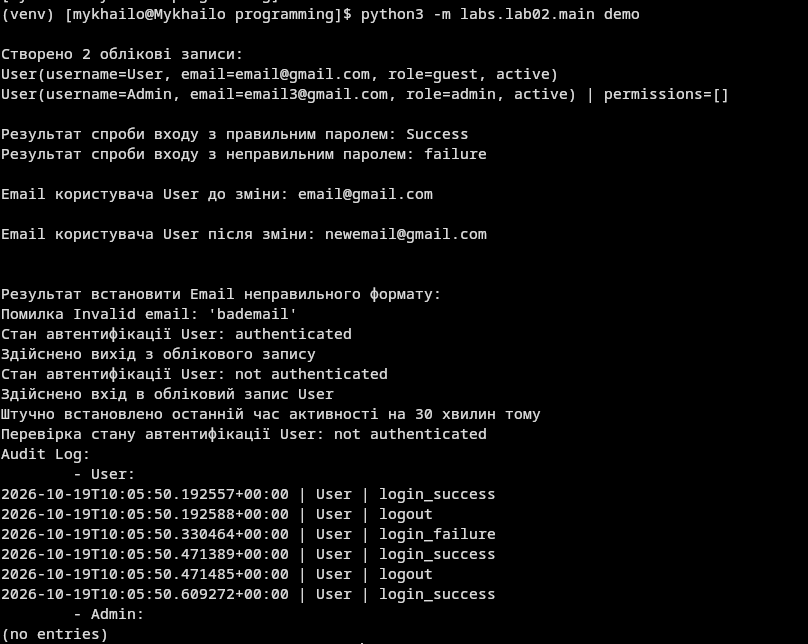
\includegraphics[width=0.7\textwidth]{lab2task1result.png}
\end{figure}
\subsection{Завдання 2: Аудитор ARP-таблицю та виявлення ARP-Spoofing}
Утиліта для аналізу зліпків ARP-кешу мережевого обладнання та виявлення аномалій.

\textbf{Функціонал:}
\begin{enumerate}
	\item Читання текстового або CSV-файлу ARP-таблиці (IP Address, MAC Address, Interface, Type).
	\item Валідація коректності IP та MAC-адрес за допомогою регулярних виразів \verb|re|.
	\item Пошук дубльованих MAC-адрес для різних IP (сигнал можливої атаки ARP-Spoofing / Man-in-the-Middle за допомогою \verb|collections.defaultdict|.
	\item Збереження виявлених конфліктів у клас даних \verb|@dataclass|.
	\item Логування критичних подій безпеки та експорт звіту в JSON.
\end{enumerate}
\textbf{CLI Аргументи:} \verb|--arp-file| (шлях), \verb|--output-json| (шлях), \verb|--detect-spoofing| (прапорець), \verb|--log-file| (шлях).

\textbf{Приклад виконання скрипта:}

\textit{Консольне виведення аудитора ARP-таблиці:}
\small\begin{lstlisting}
[INFO] Parsing ARP table snapshop from data/arp_table.csv...
[INFO] Validated 45 IP/MAC entries.

=== Validated Entries Summary ===
Valid IP/MAC Pairs: 43
Invalid Syntax: 0

=== CRITICAL SECURITY ALERTS: ARP-SPOOFING DETECTED ===
[ALERT] MAC Address Duplicate Conflict!
  MAC Address: 00:11:22:33:44:55 associated with MULTIPLE IP addresses:
  - 192.168.1.1 (Default Gateway)
  - 192.168.1.105 (Suspicious Host)
  -> POSSIBLE MAN-IN-THE-MIDDLE / ARP-SPOOFING ATTACK IN PROGRESS!

[INFO] Critical conflict lgoged to data/arp_security_alerts.json
\end{lstlisting}
\textbf{Виконання}

Лістинг task2.py:
\begin{lstlisting}
import argparse
import csv
import json
import logging
import re
from collections import defaultdict
from dataclasses import asdict, dataclass
from pathlib import Path

logger = logging.getLogger("arp_audit")

OCTET = r"(?:25[0-5]|2[0-4]\d|1\d\d|[1-9]?\d)"
IP_RE = re.compile(rf"(?:{OCTET}\.){{3}}{OCTET}")
MAC_RE = re.compile(r"(?:[0-9A-Fa-f]{2}[:-]){5}[0-9A-Fa-f]{2}")


@dataclass
class Conflict:
    mac: str
    ips: list[str]


def read_rows(path: Path) -> list[list[str]]:
    rows = []
    with path.open(encoding="utf-8", newline="") as fh:
        for line in fh:
            line = line.strip()
            if not line:
                continue

            if "," in line:
                rows.append([c.strip() for c in next(csv.reader([line]))])
            else:
                rows.append(line.split())
    return rows


def parse_arp(rows: list[list[str]]) -> tuple[list[tuple[str, str]], int]:
    valid = []
    invalid = 0
    for row in rows:
        ip = row[0] if len(row) > 0 else ""
        mac = row[1] if len(row) > 1 else ""
        if IP_RE.fullmatch(ip) and MAC_RE.fullmatch(mac):
            valid.append((ip, mac.lower().replace("-", ":")))
        elif ip.lower().replace(" ", "") in ("ip", "ipadress"):
            continue
        else:
            invalid += 1
            logger.warning("Invalid entry skipped: %s", row)
    return valid, invalid


def detect_spoofing(pairs: list[tuple[str, str]]) -> list[Conflict]:
    by_mac = defaultdict(set)
    for ip, mac in pairs:
        by_mac[mac].add(ip)
    return [Conflict(mac, sorted(ips)) for mac, ips in by_mac.items() if len(ips) > 1]


def add_arguments(parser: argparse.ArgumentParser):
    parser.add_argument("--arp-file", type=Path, required=True)
    parser.add_argument("--output-json", type=Path)
    parser.add_argument("--detect-spoofing", action="store_true")
    parser.add_argument("--log-file", type=Path)


def run(args: argparse.Namespace) -> int:
    handlers: list[logging.Handler] = [logging.StreamHandler()]
    if args.log_file:
        handlers.append(logging.FileHandler(args.log_file, encoding="utf-8"))
    logging.basicConfig(
        level=logging.INFO,
        format="[%(levelname)s] %(message)s",
        handlers=handlers,
        force=True,
    )

    logger.info("Parsing ARP table snapshot from %s...", args.arp_file)
    try:
        rows = read_rows(args.arp_file)
    except OSError as e:
        logger.error("Cannot read %s: %s", args.arp_file, e)
        return 1

    pairs, invalid = parse_arp(rows)
    logger.info("Validated %d IP/MAC entries.", len(pairs) + invalid)
    print("\n=== Validated Entries Summary ===")
    print(f"Valid IP/MAC Pairs : {len(pairs)}")
    print(f"Invalid Syntax     : {invalid}")

    conflicts = []

    if args.detect_spoofing:
        conflicts = detect_spoofing(pairs)
        if conflicts:
            print("\n=== CRITICAL SECURITY ALERTS: ARP-SPOOFING DETECTED ===")
        for c in conflicts:
            print(f"[ALERT] MAC {c.mac} associated with MULTIPLE IP addresses:")
            for ip in c.ips:
                print(f"  - {ip}")
            logger.critical("ARP spoofing: MAC %s bound to %s", c.mac, ",".join(c.ips))

    if args.output_json:
        report = {
            "valid_pairs": len(pairs),
            "invalid_entries": invalid,
            "conflicts": [asdict(c) for c in conflicts],
        }
        try:
            args.output_json.write_text(
                json.dumps(report, indent=2, ensure_ascii=False), encoding="utf-8"
            )
        except OSError as e:
            logger.error("Cannot write %s: %s", args.output_json, e)
            return 1
        logger.info("Report saved to %s", args.output_json)
    return 0
\end{lstlisting}

Результат виконання:
\begin{figure}[H]
	\centering
	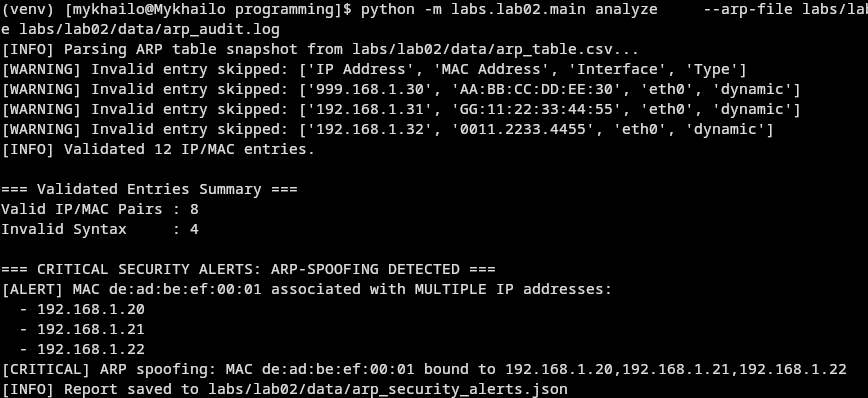
\includegraphics[width=0.7\textwidth]{lab2task2result1.png}
\end{figure}
\begin{figure}[H]
	\centering
	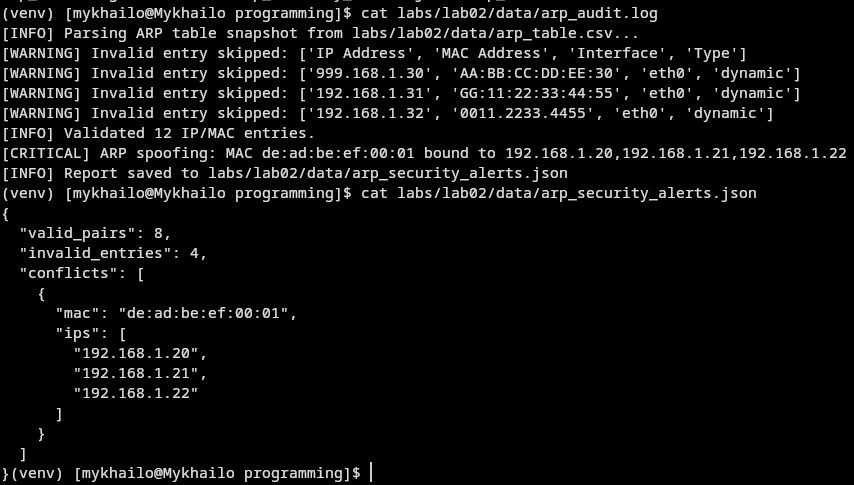
\includegraphics[width=0.7\textwidth]{lab2task2result2.png}
\end{figure}
\section{Висновок}
Під час виконання цієї лабораторної робити було засвоєно та поглиблено знання з об'єктно-орієнтованого програмування в Python, зокрема створення класів, інкапсуляція, наслідування, композиція, спеціальні методи класів та декоратори \verb|@property|, \verb|@dataclass|. Опановано роботу зі стандартною бібліотекою Python для обробки даних: маніпуляція шляхами та файлами \verb|pathlib|, робота з форматами JSON та CSV, обробка дати і часу \verb|datetime|, використання спеціалізованих структур даних \verb|collections| та регулярних виразів \verb|re|. Опановано навики побудови надійних та стійких консольних програм (CLI-утиліт): обробка винятків, валідація вхідних даних, структуроване логування подій (\verb|logging|) та розбір аргументів командного рядка (\verb|argparse|)
\end{document}
